\section{Selection}

This analysis uses the full $3.0\invfb$ of data collected by the \lhcb
experiment~\Ref{Alves:2008zz} in the years 2011 and 2012 at 7 and $8\tev$ respectively.

Candidates for the decay \btokstrdb are reconstructed, where the \db is allowed to be displaced
from the

Figure \ref{fig:lldd} shows how different tracks are categorized in \lhcb.
In the case of the decay \decay{\db}{\mumu}, the candidate dark boson could be reconstructed using
long (L) or downstream (D) tracks.
This analysis uses only the ll case, due to the fact that the trigger efficiency is low (by a
factor of at least 5, relative to that of LL) for cases using D tracks.

\begin{figure}
  \begin{center}
    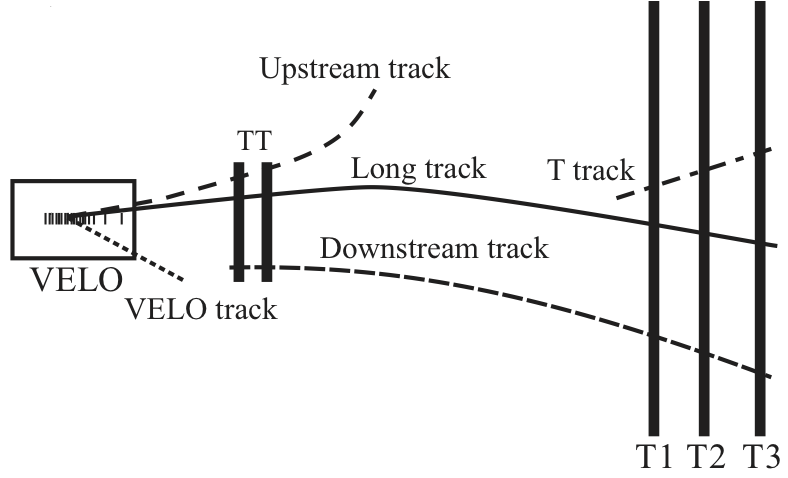
\includegraphics[width=0.48\textwidth]{track}
    \caption[Track definitions in the LHCb detector]{
      Definitions of tracks in the \lhcb detector.
      Most tracks used in analyses are classified as long tracks, but for long-lived particles
      (such as the \KS) downstream tracks are often also used to increase statistics.
    }
    \label{}
  \end{center}
\end{figure}

Simulated samples for the decay \btokstrdb are used for a variety of \mass{\db} and $\tau_\db$, as
shown in \Table{tab:db:samples}.
Also used in this analysis, are simulated events of the decays \btokstrmumu and \btojpsikstr.

\begin{table}
  \caption[Samples of simulated \btokstrdb generated for the analysis]{
    Samples of simulated \btokstrdb generated with given mass and lifetime.
    A total of 1.5 million events are generated for each sample, but only 1.5 thousand for the
    samples with a \mass{\db} of 220 and $235\mev$.
  }
  \label{tab:db:samples}
  \begin{center}
    \begin{tabular}{rccccccccccc}\toprule
      $\tau_\db$ (ps) & \multicolumn{10}{c}{\mass{\db} (MeV)} \\\midrule
      10 &&&&&&&&&2500 \\
      100 &214&220&235&250&500&800&1000&1500&2000&2500&4000 \\
      1000 &&&&250&&&&&2500 \\
      \bottomrule
    \end{tabular}
  \end{center}
\end{table}

The selection







Simulated samples are extremely important for this analysis,




It is important to remove sources of background while leaving the invariant mass of the dimuon
distribution smoothly varying, so that the assumption of local-linearity remains.

In \Sec{sec:strategy} resonances are discussed, and those where $\Gamma<5\sigmam$ must be vetoed.
For this analysis,





%\begin{figure}
  %\begin{center}
    %\includegraphics[width=0.5\textwidth]{lldd}
    %\caption{\small
      %Schematic diagram of track types in the \lhcb detector with reference to the \velo, \ttracker
      %and tracking stations one, two, and three.
      %This analysis focuses on particles decaying into a pair of long tracks.
    %}
    %\label{fig:lldd}
  %\end{center}
%\end{figure}
%
%\subsection{Reconstruction and Stripping}
%The offline selection begins using the {\tt B2KpiX2MuMuDarkBosonLine}
%stripping line for \ll candidates
%from {\tt Stripping20r0p3} ({\tt Stripping20r1p3} for 2011 data).
%%Candidates constructed from a pair of downstream  (\dd) muons were considered but found not to be
%%useful, please refer to Appendix~\ref{sec:lldd} for detils.
%The selection criteria applied in these lines are outlined in \Tab{tab:stripping}.
%The variable {\tt DOCA} is defined as the distance of closest approach between any two pairs of
%tracks in the candidate.
%Also used is the variable \chisqfd, which is the change in vertex \chisq when the signal candidate
%tracks are associated with the PV in the vertex fit.
%Candidates are reconstructed using {\tt DecayTreeFitter}, where daughter particles are constrained
%such that the reconstructed $\kpi\mumu$ invariant mass, $m(\kpi\mumu)$, is equal to the nominal \Bd mass.
%All references to $m(\db)$, $m(\Kstar)$ or $\tau(\db)$ are to the values after this vertex fit
%has been performed.
%
%
%

%\begin{table}
  %\caption{\small
    %Stripping cuts, pions are taken from {\tt StdAllNoPIDsPions}, kaons from {\tt StdAllNoPIDsKaons}
    %and muons are from {\tt StdAllLooseMuons}.
    %While the $B$ mass is constrained in the fit, the selection makes a cut on the unconstrained
    %mass.
    %%The variable {\tt DOCA} is defined as the distance of closest approach between any two pairs of
    %%tracks in the candidate.
  %}
  %\label{tab:stripping}
  %\begin{center}
    %\begin{tabular}{llcrl}\toprule
      %Candidate & \multicolumn{4}{c}{Cut} \\\midrule
      %$B$
      %& $\chisqvtx/\ndf$          & $<$ & 25   \\
      %& \chisqip                  & $<$ & 50   \\ % BPVIPCHI2
      %& $\tau$                    & $>$ & 0.2 & ps  \\
      %& $m$                       & $\in$ & $[4800, 5800]$  & MeV \\
      %& \pt                       & $>$ & 1000    & MeV   \\
      %& $\cos\theta_\mathrm{dir}$     & $>$ & 0 \\
      %\midrule
      %\db
      %& $\chisqvtx/\ndf$          & $<$ & 10   \\ % VCHI2DOF
      %%& $\chisqvtx/\ndf$           & $<$ & 10 & 25   \\ % VCHI2DOF
      %& $\chisqfd$                & $<$ & 25   \\
      %& \pt                       & $>$ & 250  & MeV \\
      %%& \pt (MeV)                  & $<$ & 250 & $0$ \\
      %& {\tt DOCA}                & $<$ & 0.2 & mm \\
      %& {\tt DOCA} \chisq         & $<$ & 25  &    \\
      %\midrule
      %Tracks
      %& $\chisqtrk/\ndf$          & $<$ & 3    \\
      %& $\min(\chisqip)$                  & $>$ & 9    \\ % MIPCHI2DV
      %& $\mathcal{P}_\mathrm{gh}$ & $<$ & 0.3  \\
      %\midrule
      %$K$, $\pi$
      %& \pt                       & $>$ & 250  & MeV \\
      %& $p$                       & $>$ & 2000 & MeV \\
      %& \chisqip                  & $>$ & 9 \\
      %$K$
      %& {\tt ProbNNK}             & $>$ & 0.1  \\
      %$\pi$
      %& {\tt ProbNNpi}            & $>$ & 0.2  \\
      %$\mu$
      %& \pt                       & $>$ & 100  & MeV \\
      %& {\tt PIDmu}               & $>$ & -5   \\
      %\bottomrule
    %\end{tabular}
  %\end{center}
%\end{table}




%\subsection{Triggering}
%The triggers used are given in \Tab{tab:triggers}.  All trigger lines with non-negligible efficiency are used.
%Only {\tt TOS} candidates are used in this analysis for two reasons: (1) the ratio of trigger
%efficiency for the SM \decay{\Bd}{\Kstarz\mumu} to that of (possibly displaced) \db mode enters
%into the limits and, thus, must be precisely determined and (2) the use of {\tt TIS} events would
%come with a substantial enhancement of the di-$b$-hadron backgrounds.
%The few percent gain in signal efficiency obtained using {\tt TIS} is not worth the increase in the di-$b$-hadron backgrounds.
%
%\begin{table}
  %\begin{center}
    %\caption{\small
      %Trigger lines used for the selection, the exact requirement is that a
      %candidate must be TOS on at least one trigger line in each trigger level.
    %}
    %\label{tab:triggers}
    %\begin{tabular}{llll}\toprule
      %Level & \multicolumn{3}{c}{Trigger line} \\\midrule
      %{\tt L0} % with decision on the end
      %& {\tt L0Hadron} & {\tt L0Muon} & {\tt L0DiMuon} \\\midrule
      %{\tt HLT1}
      %& {\tt Hlt1TrackAllL0} & {\tt Hlt1TrackMuon} & {\tt Hlt1DimuonLowMass} \\\midrule
      %%& {\tt Hlt1MuTrack} \\
      %{\tt HLT2}
      %& {\tt Hlt2TopoMu2BodyBBDT} & {\tt Hlt2TopoMu3BodyBBDT} & {\tt Hlt2TopoMu4BodyBBDT} \\
      %& {\tt Hlt2Topo2BodyBBDT} & {\tt Hlt2Topo3BodyBBDT} & {\tt Hlt2Topo4BodyBBDT} \\
      %& {\tt Hlt2SingleMuon} & {\tt Hlt2DiMuonDetached} \\ % & {\tt Hlt2MuTrack} \\
      %\bottomrule
    %\end{tabular}
  %\end{center}
%\end{table}
%
%
%
%
%\subsection{Preselection}
%After the stripping and triggering stages, a loose preselection is applied (see \Tab{tab:presel}).
%The data sample is further purified using a multivariate algorithm, which is discussed in the
%following subsection.
%The preselection places cuts on topological quantities the combined efficiency of which is
%$\sim90\%$ on all simulated samples.
%Loose hadron particle identification requirements and a $m(\kpi)$ cut are also made to remove any
%candidates clearly inconsistent with the decay $\Kstarz\!\to \kpi$.
%Since the \db lives an unknown amount of time, muons originating from another Primary Vertex (PV).
%To suppress this possibility, the transverse flight distance, $FD_T$, of the
%\db is required to be at least $0.1\mm$, this cut is close to $100\%$ efficient for all simulated
%samples.
%The $FD_T$ is defined to be the distance in the $x-y$ plane, between the PV and the decay vertex of
%the \db.
%This suppresses even the case where the second PV is not reconstructed
%since the vast majority of all $pp$ collisions happen less than 0.1\mm from the nominal beam
%line.
%%The distribution of the radial $PV$ positions is shown in \Fig{fig:pv}.
%
%In \Sect{sec:strategy} it is briefly mentioned that the observed signal yields will be normalized
%with respect to the SM decay \btokstrmumu.
%Specifically the \qsq range $1.1<\qsq<6.0\gevgev$ will be used, because theoretical and
%experimental uncertainties are low in this region.
%Here, \qsq is defined to be the invariant mass of the dimuon pair, squared.
%
%
%\begin{table}
  %\caption{\small
    %Preselection cuts.
  %}
  %\label{tab:presel}
  %\begin{center}
    %\begin{tabular}{lccrl}\toprule
      %Variable & \multicolumn{3}{c}{Cut}\\
      %\midrule
      %$\theta_\mathrm{dir}(\Bd)$ &$<$& 0.03 & rad \\
      %$\chisqvtx(\Bd)$ &$<$& 15 \\
      %$\chisqip(\Bd)$ &$<$& 10 \\
      %$\dllkpi(K)$&  $>$ & -5 \\
      %$\dllkpi(\pi)$&  $<$ & 25 \\
      %$\dllkpi(K)-\dllkpi(\pi)$ & $>$ & 10 \\
      %$|m(\Kp\pim)-895.6|$ & $<$ & 100 & MeV \\
      %$FD_T(\db)$ & $>$ & 0.1 & mm \\
      %{\tt isMuon}($K,\pi$) && {\tt False} \\
      %\bottomrule
    %\end{tabular}
  %\end{center}
%\end{table}
%




%\subsection[Mass of \Bd candidates]{Mass of $\boldsymbol{\Bd}$ candidates}
%\label{ssec:sel:massb}
%As mentioned above, all masses in this analysis are computed using {\tt DecayTreeFitter}, where the
%mass of the \Bd candidate is constrained to the world average value in the vertex fit~\cite{PDG2012}.
%The analysis is performed on all \Bd candidates that fall within $150\mev$ of the nominal \Bd
%mass~\cite{PDG2012}, where the mass is the mass from the unconstrained vertex fit (the upper sideband of
%which is used for to train the multivariate selection, which is described below).
%A tighter criteria is placed on the \Bd mass to select the final sample of candidates to use in the \db search.
